\glsreset{iot}
\glsreset{fdma}

\chapter{Introduction}
\label{sec:introduction}
Sigfox is a commercial \gls{lpwan} technology developed and marketed by the French company ``Sigfox \gls{sa}'' based in Toulouse (in the following, sometimes also just referred to as ``Sigfox'' or ``Sigfox company'').
It aims to complement traditional wireless network technologies by specifically targeting low-power \gls{iot} devices and providing inexpensive and long-range (``up to the horizon'', \cite[Section 3.3]{phyandmac}) connectivity at the expense of limited message lengths.
As of September 2018, Sigfox is under rollout in many countries globally, while best coverage is currently found in Western Europe \cite{coveragemap}.

\FloatBarrier
\section{The Emergence of LP-WAN networks}
An increasing number of often battery-powered devices, commonly referred to under the umbrella term ``\gls{iot} devices'', need to be connected to the internet.
Application areas for \gls{iot} devices are manifold; sensor networks, asset tracking, fleet management, agriculture and buzz-words like ``Smart City'' are just some of many frequently mentioned examples.

Challenges arising with this trend are, among others, ensuring the security of \gls{iot} devices and providing connectivity to the internet.
The latter is especially difficult if power constraints are in place and data has to be transmitted wirelessly.
Traditional wireless communication protocols are often unsuited for this new field of application \cite{iot_protocol_overview}.
WiFi, Bluetooth and ZigBee are relatively inexpensive, but only provide a short range of typically up to 100m \cite[Table 1]{iot_protocol_overview}.
Cellular networks (\gls{gsm}, \gls{umts}, \gls{lte} and the like) on the other hand do not have the same problem, but are associated with a high power consumption on client devices and higher costs which makes them inappropriate for \gls{iot} applications \cite{lpwan_comparison}.

\glspl{lpwan} address these issues by providing long-range, low-cost and low-power connectivity at the expense of low data rates.
Currently, the three main competitors in this field as identified by \cite[Section 1]{lpwan_comparison} are LoRa, Sigfox and the \gls{3gpp}'s \gls{nbiot}.
While \gls{nbiot} is supported by many mobile carriers, its deployment has been significantly delayed since specifications were released as late as June 2016 and because its radio range is the shortest of all three standards.
This left a void in the market for \gls{lpwan} solutions which allowed LoRa and Sigfox to achieve considerable coverage and mature in the meantime \cite[Section 3.5]{lpwan_comparison}.

A detailed classification of Sigfox and a comparison to competing protocols would be outside the scope of this document.
Broadly speaking, Sigfox can be seen as a technology with extremely low data rates and payload sizes, even in the context of other \gls{lpwan} protocols.
More nuanced comparisons with other \gls{lpwan} networks and traditional wireless technologies that are often employed in the \gls{iot} are made in \cite{lpwan_comparison} and \cite{iot_protocol_overview}.

\FloatBarrier
\section{Sigfox as an LP-WAN Technology}
\subsection{License-free Bands}
Generally, parts of the radio spectrum are allocated to specific communication services such as television and radio broadcasting, cellular networks or satellite communications.
Frequency allocations are typically performed by governmental entities and are usually associated with high costs to companies or individuals requesting the exclusive use of a spectral band.
Exceptions to this are provided through the license-free so-called \gls{ism} radio bands (worldwide) and the European \gls{srd} bands.
These bands can be used by anyone without any need for registration for a more loosely defined set of applications under less tight restrictions, e.g. a limited duty cycle and limited maximum transmission power.
\Cref{fig:srd_bands} illustrates limitations for some selected license-free \gls{srd} bands that might be suitable for the operation of an \gls{lpwan} network in Europe.
\Cref{fig:srd_bands} does not show, for instance, limitations on the type of application that the unlicensed bands are designated for and also does not show all possible \gls{srd} bands.
Refer to \cite{bnetza_srd} for the complete details.

\begin{figure}[h]
	\centering
	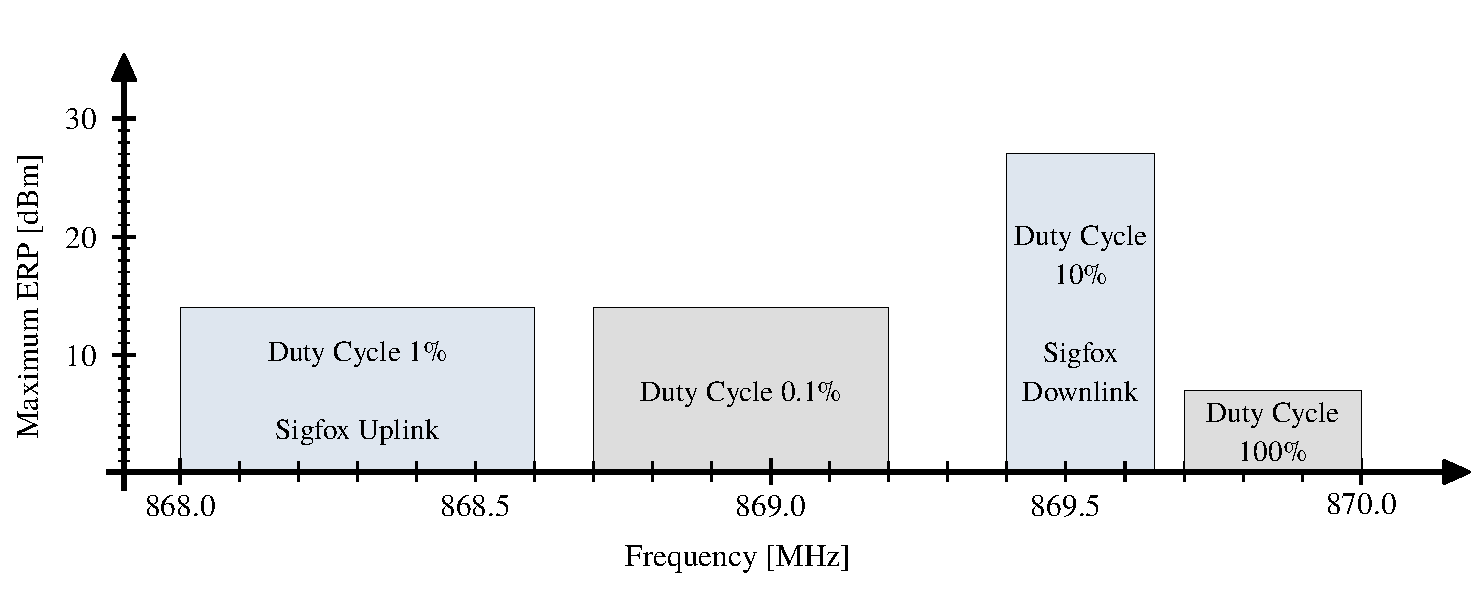
\includegraphics[width=1.0\textwidth]{fig/srd_bands.pdf}
	\caption{Some unlicensed bands in the 868.0 MHz to 870.0 MHz range and their maximum \gls{erp} and duty cycle, based on ETSI EN 300 220-2 V3.1.1 / Bundesnetzagentur \gls{srd} regulations \cite{bnetza_srd}}
	\label{fig:srd_bands}
\end{figure}

\FloatBarrier
Enabled by advancements in \gls{rf} technology such as better filters for \gls{unb} communication, some \gls{lpwan} providers such as LoRa and Sigfox have opted to operate their networks in license-free bands avoiding the costly acquisition of radio spectrum.
This implies though, that their base stations as well as all client devices have to conform to official regulations concerning the use of these bands.

\subsection{Ultra-Narrowband Technology}
Legal regulations for license-free bands usually specify a limited maximum transmission power per device, which limits the maximum range that is achievable.
They do typically not, however, limit the spectral power density, so that legally, transmission power can be concentrated in a very narrow frequency range improving spectral efficiency.
Through the use of accurate filtering at the receiver, the effect of noise on the communication system can be limited so that long radio ranges can be achieved \cite[Section 3.3]{phyandmac} \cite[Section 2.1]{lpwan_comparison}.
This way, long-range wireless communication networks can be built in license-free bands while respecting legal limitations.

Additionally, \gls{unb} technology is characterized through low power consumption \cite[Section 2.1]{lpwan_comparison}, a low chance of transmission collisions (see also \Cref{sec:ul_repetitions}), but also through low data rates, as illustrated by this simple consideration:
For an ideal $\frac{\sin \left( x \right)}{x}$ pulse shaping at a symbol rate $R_s$, a bandwidth of $B = R_s$ is used.
Since no modulation scheme can surpass ideal pulse shaping, if only a limited bandwidth $B$ is available, the symbol rate cannot exceed $R_s = B$.

\FloatBarrier
\section{Sigfox Network Architecture}
\begin{figure}[h]
	\centering
	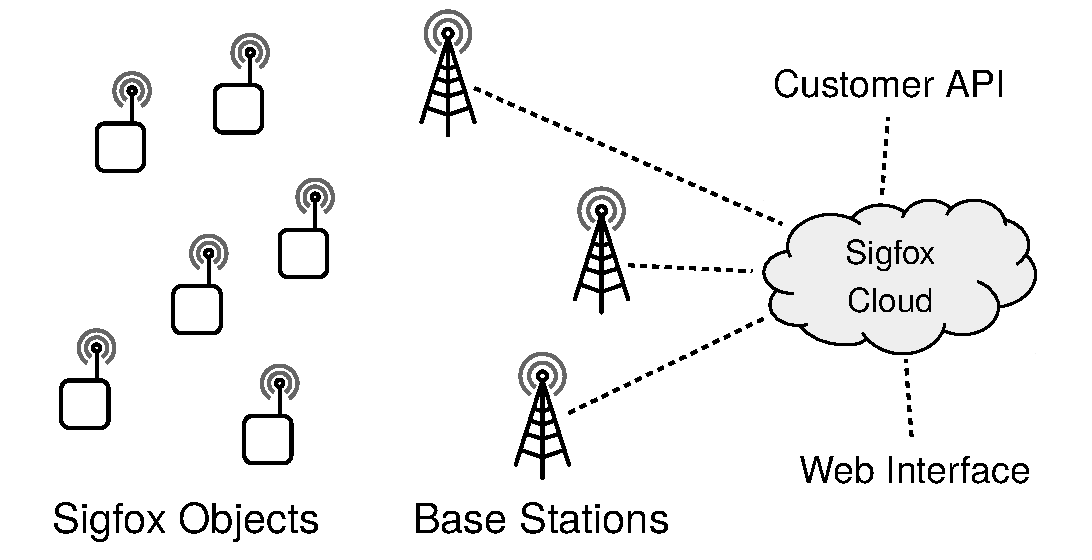
\includegraphics[width=0.8\textwidth]{fig/NetworkLayout.pdf}
	\caption{Basic architecture of the Sigfox network}
	\label{fig:network_architecture}
\end{figure}

As illustrated in \Cref{fig:network_architecture}, the Sigfox network consists of two types of devices: Client devices called \textbf{Sigfox objects} (naming adapted from \cite{sigfox_tech}) and \textbf{Sigfox base stations}.
Sigfox objects are typically \gls{iot} devices owned by customers that pay a subscription fee to the Sigfox \gls{sa} company which provides base stations and cloud backend.
The network is designed as a simple star topology, that is the objects directly communicate with the base stations over a radio link.
Bidirectional communication is supported, i.e. Sigfox objects can send ``uplinks'' to a base station or receive ``downlinks'' from it.
The payload size of uplinks is limited to 12 bytes at maximum and that of downlinks to 8 bytes with the total number of uplinks and downlinks per day also being restricted based on the customer's subscription plan.
Moreover, Sigfox objects do not need to be active except when sending or receiving a message as no previous synchronization with the network before transmitting data is required.
Neither does the network signal any acknowledgement of successful uplinks.
Sigfox objects also do not listen for downlinks except for during a predefined time frame after having transmitted an uplink that explicitly requests a downlink, so downlinks can only occur after an object has initiated an uplink.
Contrary to common cellular radio protocols, a Sigfox object is not even associated with any specific base station prior to sending an uplink, but the uplink is received by whatever stations happen to detect it (this principle is called cooperative reception \cite[Section 3.3]{sigfox_tech}).
Base stations are connected to a central ``Sigfox Cloud'', a collection of servers managed by Sigfox \gls{sa}, over point-to-point links.
Ultimately, Sigfox customers can create user accounts with Sigfox \gls{sa} and register their own Sigfox objects to retrieve the messages sent by them using a web interface to the Sigfox cloud or with an \gls{api}.
Each Sigfox object is identified by its unique device ID and a \gls{pac}, but the latter is only used once for registration of the device with the user's Sigfox account.

\FloatBarrier
\section{Motivation}
Security is a key challenge for \gls{iot}.
Many small devices that possibly gather sensitive information broaden the attack surface on businesses that employ them and are sometimes financially dependent on them \cite[Executive Summary]{sigfox_security_whitepaper}.
On the other side, market forces cause manufacturers of \gls{iot} devices to compromise on their security due to the demand for very low-cost solutions.

One of the key selling points for Sigfox is its alleged security.
Since, in contrast to WiFi devices, Sigfox objects are not directly connected to the internet, they are claimed to be protected by a firewall that is inherent to the Sigfox network design.
Sigfox also promises a secure radio protocol design including message integrity checking and replay protection \cite{sigfox_security_whitepaper}, but since Sigfox does not publish protocol specifications, there is no way for security researchers to verify their claims.
The goal of this work is therefore to understand the Sigfox radio protocol so that its security can be verified independently.

\FloatBarrier
\section{Related Work}
Just like Sigfox's, LoRa's physical layer is also proprietary and closed-source.
Reverse engineering work on LoRa, similar to what this specifications document does for Sigfox, has been performed by M. Knight and B. Seeber.
Their success has been documented in \cite{lora_gr} or more informally, but extensively in \cite{lora_poc}, partly inspiring this work.

Some initial reverse engineering of parts of the Sigfox uplink has been conducted by technology blogger P. Pinault \cite{disk91radioprotocol}.
The publication of his work substantially accelerated work on the open Sigfox stack.

\vspace{-0.2cm}
\FloatBarrier
\section{Overview and Limitations}
\vspace{-0.2cm}
This document is divided into four main chapters:
In this introductory section, the basic concepts of Sigfox and \gls{lpwan} technology in general have been outlined and a quick classification of Sigfox in the broader context of \gls{iot} radio protocols was given.
In \Cref{sec:uplink}, Sigfox's uplink communication from object to base station will be investigated and in \Cref{sec:downlink}, the analysis of Sigfox's communication from base station to object (downlink) will be presented.
In \Cref{sec:conclusion}, some final thoughts and ideas for further research topics will be outlined.
Uplink and downlink chapters conclude with a section on some preliminary security assessment which has been carried out based on suspected protocol specifications obtained from the analysis, but without consideration of professionals in the field of cryptography. 

As part of this work, an open source implementation of the described Sigfox network stack has been created.
It consists of a library called \texttt{librenard} as well as its command line front end called \texttt{renard}, both written in the C programming language.
\texttt{renard} can decode and encode Sigfox up- and downlinks, but does not take care of physical layer modulation / demodulation and takes digital (hexadecimally encoded) data as in- and output instead.
The separate library \texttt{librenard} was created with the intent to make the encoding / decoding functionality portable to different platforms such as microcontrollers so that Sigfox connectivity can be embedded in various applications without requiring a branded Sigfox modem or relying on closed-source binary blobs.
More information on how to obtain and use \texttt{librenard} and \texttt{renard} is given in \Cref{sec:renard_usage}.

For each individual, technical aspect of uplink and downlink, a brief introduction to the topic is provided, followed by a subsection on the assumed realization of that aspect by Sigfox.
Subsequently, aspects of an alternative network stack that is implemented in \texttt{renard} or \texttt{librenard} are presented.
In a final subsection labelled ``Results'', it is confirmed whether the findings on the technical aspect are correct and how this information can be applied.
Additionally, some remarks about protocol design choices and suggestions for areas of further research may be made.
The methods used for protocol reconstruction are omitted from the individual protocol aspects to not clutter the explanations, but are briefly summarized in \Cref{sec:analysismethods}.

It has to be noted that the presented information about the protocol may be incomplete.
While all statements that will be made have been carefully tested and verified, it is unknown whether this document describes the complete specification of uplink and downlink or whether significant portions have been overlooked.
